% PrototypeDevelopmentLifecycle.tex
\subsection{Lifecycle}
This section provides an overview of the Prototype Development Lifecycle.

\subsubsection*{Conceptualization and Requirements Definition}
\begin{itemize}
  \item The prototype must have four photodiodes in an xy pattern with respective circuitry required to output ~0-5 Volts that will be read by an Arduino based Data Acquisition System (DAQ). The circuit must be able to react to light intensity changes, however the change will be at low frequency ( below 1Hz) as a satellite attitude is considered to change only gradually.
  \item While the prototype may not have a high accuracy, it is hoped that it will be enough to measure light position changes roughly, even if at a low accuracy of ~10° or ~20° but this will remain to be seen.  
  \item The prototype within the scope of this paper will show the ability to detect the position of light at normal room conditions, therefore it does not need to withstand temperature changes or radiation that a final product would require if deployed in space.
  \item Interface requirements: the prototype electrical output needs to be compatible with the Arduino Analog to Digital Converter (ADC) input. Therefore, the signal shall not go below 0 Volts or exeed 5 volts. 
  \item Size and weight are not of high importance, but the device must fit in the testing equipment, which is the Renewable Energy Demonstrator arch. Preferably a height not higher than 5cm.
\end{itemize}

\subsubsection*{Theoretical Design}
The prototype will be composed of three parts: a stripboard containing the components for the amplification circuit,  a 3D printed Photodiode enclosure which will allow placing the photodiodes in the correct positions, as the photodiodes have the legs at a smaller distance than the stripboard, and need to be placed quite close to eachother, with the third part being the Arduino based DAQ. 
% DIAGRAM MAYBE IN FRITZING???
%
% Reference in teh text above
% \begin{figure}[htbp] %h-ere t-op b-ottom p-page (separte) -good to allow all htbp to give the compiler more options
%   \centering
%   \includegraphics[width=0.8\textwidth]{chapters/methodology/prototype/fritzingdiagram??.png}
%   \caption{Rough Diagram of Photodiode Array with Apertures}
%   \label{fig:diodeApertureDiagram}
% \end{figure}
The third part to the 


\paragraph{Sun Sensor Geometry and Aperture Design} was decided to be in a T shape, providing an x-y layout with two photodiodes in the x direction and two photodiodes in the y direction. Combined with an aperture design that covers one half of each diode, as represented in Figure \ref{fig:diodeApertureDiagram}. This configuration is similar to Ortega et al. in their paper attempting to miniaturize a two axis Sun Sensor\cite{RefWorks:ortega2010miniaturized}.

% Photodiode Aperture Diagram
%
\begin{figure}[htbp] %h-ere t-op b-ottom p-page (separte) -good to allow all htbp to give the compiler more options
    \centering
    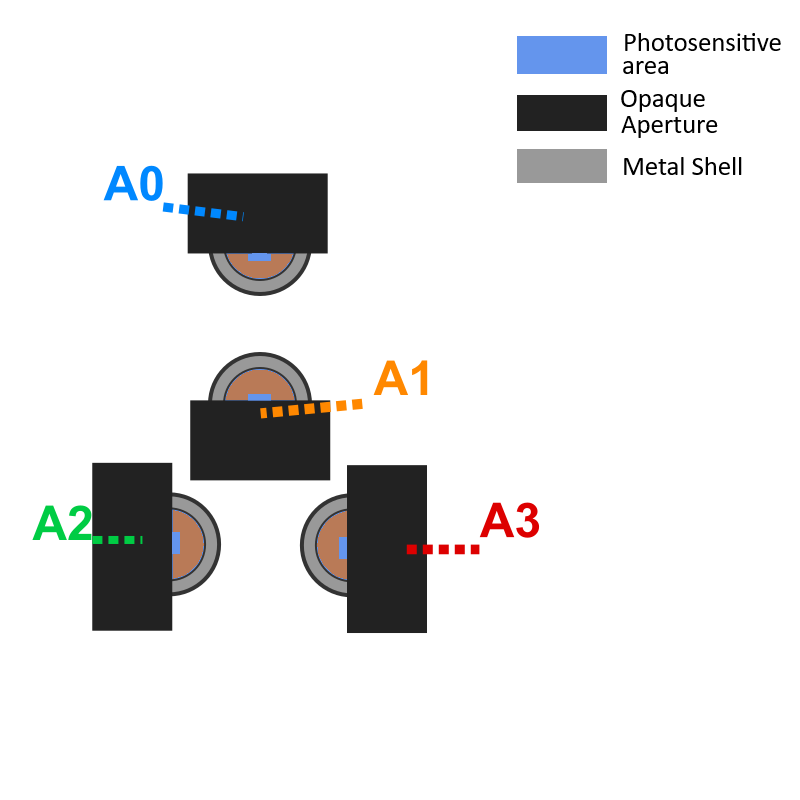
\includegraphics[width=0.6\textwidth]{chapters/methodology/prototype/diodeApertureDiagram.png}
    \caption{Diagram of Photodiode Array with Apertures}
    \label{fig:diodeApertureDiagram}
\end{figure}


\subsubsection*{Component Selection}
The components chosen for the design of the prototype are detailed below. They were first placed on a BreadBoard and tests were performed to ensure the functionality of the circuit before moving them to a stripboard which would ensure the components are phisically more stable and reduce the chance of faulty connectoins. Therefore, the same components were used for both BreadBoard and StripBoard prototyping. The circuit design and testing is gone into more detail in Section \ref{subsec:SignalConditioningCircuitry}. 

% components for Amplification Circuit
\begin{table}[htbp]
  \centering
  \begin{threeparttable}
    \caption{Electrical Components Used in Amplification Circuit}
    \label{tab:components_list_stripboard}
    \begin{tabular}{lccc}  
      \toprule
      \textbf{Component Type} & \textbf{Comp. Part Name} & \textbf{Component Value} & \textbf{Amount} \\
      \midrule
      Op-Amp & TI LM324-N & -- & 2 \\
      Photodiode & Hamamatsu S5971 & -- & 4 \\
      Resistor & -- & 1 M$\Omega$ & 4 \\
      Resistor & -- & 150 k$\Omega$ & 4 \\
      Resistor & -- & 10 k$\Omega$ & 4 \\
      Capacitor & -- & 1 $\mu$F & 4 \\
      Stripboard & Veroboard & -- & 1 \\
      Screw terminal block & -- & 2-input & 3 \\
      \bottomrule
    \end{tabular}
    
  \end{threeparttable}
\end{table}

% TABLE COMPONENTS DAQ
\begin{table}[htbp]
  \centering
  \begin{threeparttable}
    \caption{Components Used for DAQ System}
    \label{tab:daq_components}
    
    \begin{tabular}{lccc}  
      \toprule
      \textbf{Component Type} & \textbf{Component Part Name} & \textbf{Component Value} & \textbf{Amount} \\
      \midrule
      Microcontroller & Arduino Uno & -- & 1 \\
      Cable & USB cable & -- & 1 \\
      Computer & Laptop/Python & -- & 1 \\
      \bottomrule
    \end{tabular}
    
  \end{threeparttable}
\end{table}

\paragraph{Photodiodes} were researched and several options were found, most of which were quite expensive, such as 2D PSD type sensors like the Hamamatsu S5990 but were both prohibitivly expensive and Surface Mount Device style (SMD), which would have been harder to prototype but would allow for much higher resolutions, while also complicating the project due to the more complex nature of PSDs. A decision was made to base the project on 1D photodiodes, and four Hamamatsu S5971 were purchased, which offered a good compromise in price and specifications: 

\begin{table}[h]
  \centering
  \caption{S5971 Photodiode Specifications}
  \begin{tabular}{|l|c|}
  \hline
  \textbf{Parameter} & \textbf{Value} \\
  \hline
  Spectral response range ($\lambda$) & 320 to 1060 nm \\
  \hline
  Peak sensitivity wavelength ($\lambda_p$) & 920 nm \\
  \hline
  Photosensitivity S (A/W) at $\lambda_p$ & 0.64 \\
  \hline
  Photosensitivity S (A/W) at 780 nm & 0.55 \\
  \hline
  Photosensitivity S (A/W) at 830 nm & 0.6 \\
  \hline
  Short circuit current Isc & 1.0 $\mu$A \\
  \hline
  Dark current Id (Typical) & 0.07 nA$^{*3}$ \\
  \hline
  Dark current Id (Maximum) & 1 nA$^{*3}$ \\
  \hline
  Cutoff frequency fc & 0.1 GHz$^{*3}$ \\
  \hline
  Terminal capacitance Ct (f=1 MHz) & 3 pF$^{*3}$ \\
  \hline
  Noise equivalent power NEP ($V_R$=10 V, $\lambda$=$\lambda_p$) & 7.4 $\times$ 10$^{-15}$ W/Hz$^{1/2}$ \\
  \hline
  \end{tabular}
  \begin{tablenotes}
  \small
  \item[*3] $V_R$ = 10 V
  \end{tablenotes}
  \end{table}

Although the higher versions such as S5972-3 have better specifications, such as frequency cutoff of 1GHz and lower Dark current, these were not needed for our project, higher frequency cut off not needed due the static nature of the light source and dark current, while it could affect a case where one of the diodes is fully in the dark, a voltage offeset would be noticeable, but with a voltage resolution restricted by the Arduino DAQ to 4.88mV/step, it was deemed acceptable:
\begin{equation} \label{eq:darkCurrentOffset}
  \begin{split}
V_\text{offset-TIA} &= I_d \times R_f \\
&= 0.07 \text{ nA} \times 1 \text{ M}\Omega \\
&= 70 \text{ }\mu\text{V}
  \end{split}
\end{equation}
\addequation{DC Offset Voltage at TIA Output Due to Dark Current}
\begin{equation} \label{eq:totalDCoffset}
  \begin{split}
V_\text{offset-total} &= V_\text{offset-TIA} \times \text{Gain}_\text{post-amp} \\
&= 70 \text{ }\mu\text{V} \times 16 \\
&= 1.12 \text{ mV}
  \end{split}
\end{equation}
\addequation{Total DC Offset After Post-Amplification}
Equation \ref{eq:totalDCoffset} above shows the final dark current would be a maximum of 1.12mV which is below what the ADC can detect. 

\paragraph{\acf{OpAmp}} choice was once again not a complicated choice due to the same arguments mentioned above re. photodiode selection: low frequency signal and reduced DAQ resolution. The LM324-N is a low-cost \ac{OpAmp} which provides acceptable performance. 
%
%           ~~~   OPAMP SPECIFICATION TABLE    ~~~
%
\begin{table}[htbp]
  \centering
  \caption{Operational Amplifier Specifications}
  \begin{tabular}{|l|c|}
  \hline
  \textbf{Parameter} & \textbf{Value} \\
  \hline
  DC Voltage Gain & 100 dB \\
  \hline
  Unity Gain Bandwidth & 1 MHz \\
  \hline
  Supply Voltage Range (Single) & 3 V to 32 V \\
  \hline
  Supply Voltage Range (Dual) & $\pm$1.5 V to $\pm$16 V \\
  \hline
  Supply Current & 700 $\mu$A \\
  \hline
  Input Bias Current & 45 nA \\
  \hline
  Input Offset Voltage & 2 mV \\
  \hline
  Input Offset Current & 5 nA \\
  \hline
  Input Common-Mode Voltage Range & Includes Ground \\
  \hline
  Differential Input Voltage Range & Equal to Supply Voltage \\
  \hline
  Output Voltage Swing & 0 V to V$^{+}$ - 1.5 V \\
  \hline
  \end{tabular}
  \begin{tablenotes}
  \small
  \item Internally frequency compensated for unity gain
  \item Temperature compensated
  \end{tablenotes}
\end{table}
The advantages in choosing this \ac{OpAmp} is its ability to function on a single pole Power Supply, it is rather cheap while still offering 1MHz Unity Gain Bandwidth and is recommended for DC Gain which the type of signal our project aims to amplify. For example, the slew-rate characteristic is not mentioned on the datasheet because it is aimed at low frequency operation.


%
%           ~~~   BreadBoard Testing subsection   ~~~
%
\subsubsection*{BreadBoard Testing}

Once the circuit design was completed as seen in Figure  \ref{fig:AltiumDis}, the components were placed on a BreadBoard to test the real circuit, as seen in Figure \ref{fig:BreadBoardPhoto}. 
There were several iterations, at first with only the \ac{TIA} and one photodiode- a design that when tested, resulted in a low Voltage output when testing with only the \ac{LED} light from the \ac{RED} testbench. This is due to the low light power of \acp{LED}. A decision was made to add a secondary amplification circuit which raised the Voltage to a maximum 5V as designed. Further details on design in Section \ref{subsec:SignalConditioningCircuitry}. The final BreadBoard design can be found in Figure \ref{fig:BreadBoardPhoto}.



% BreadBoard photo
%
\begin{figure}[htbp] %h-ere t-op b-ottom p-page (separte) -good to allow all htbp to give the compiler more options
  \centering
  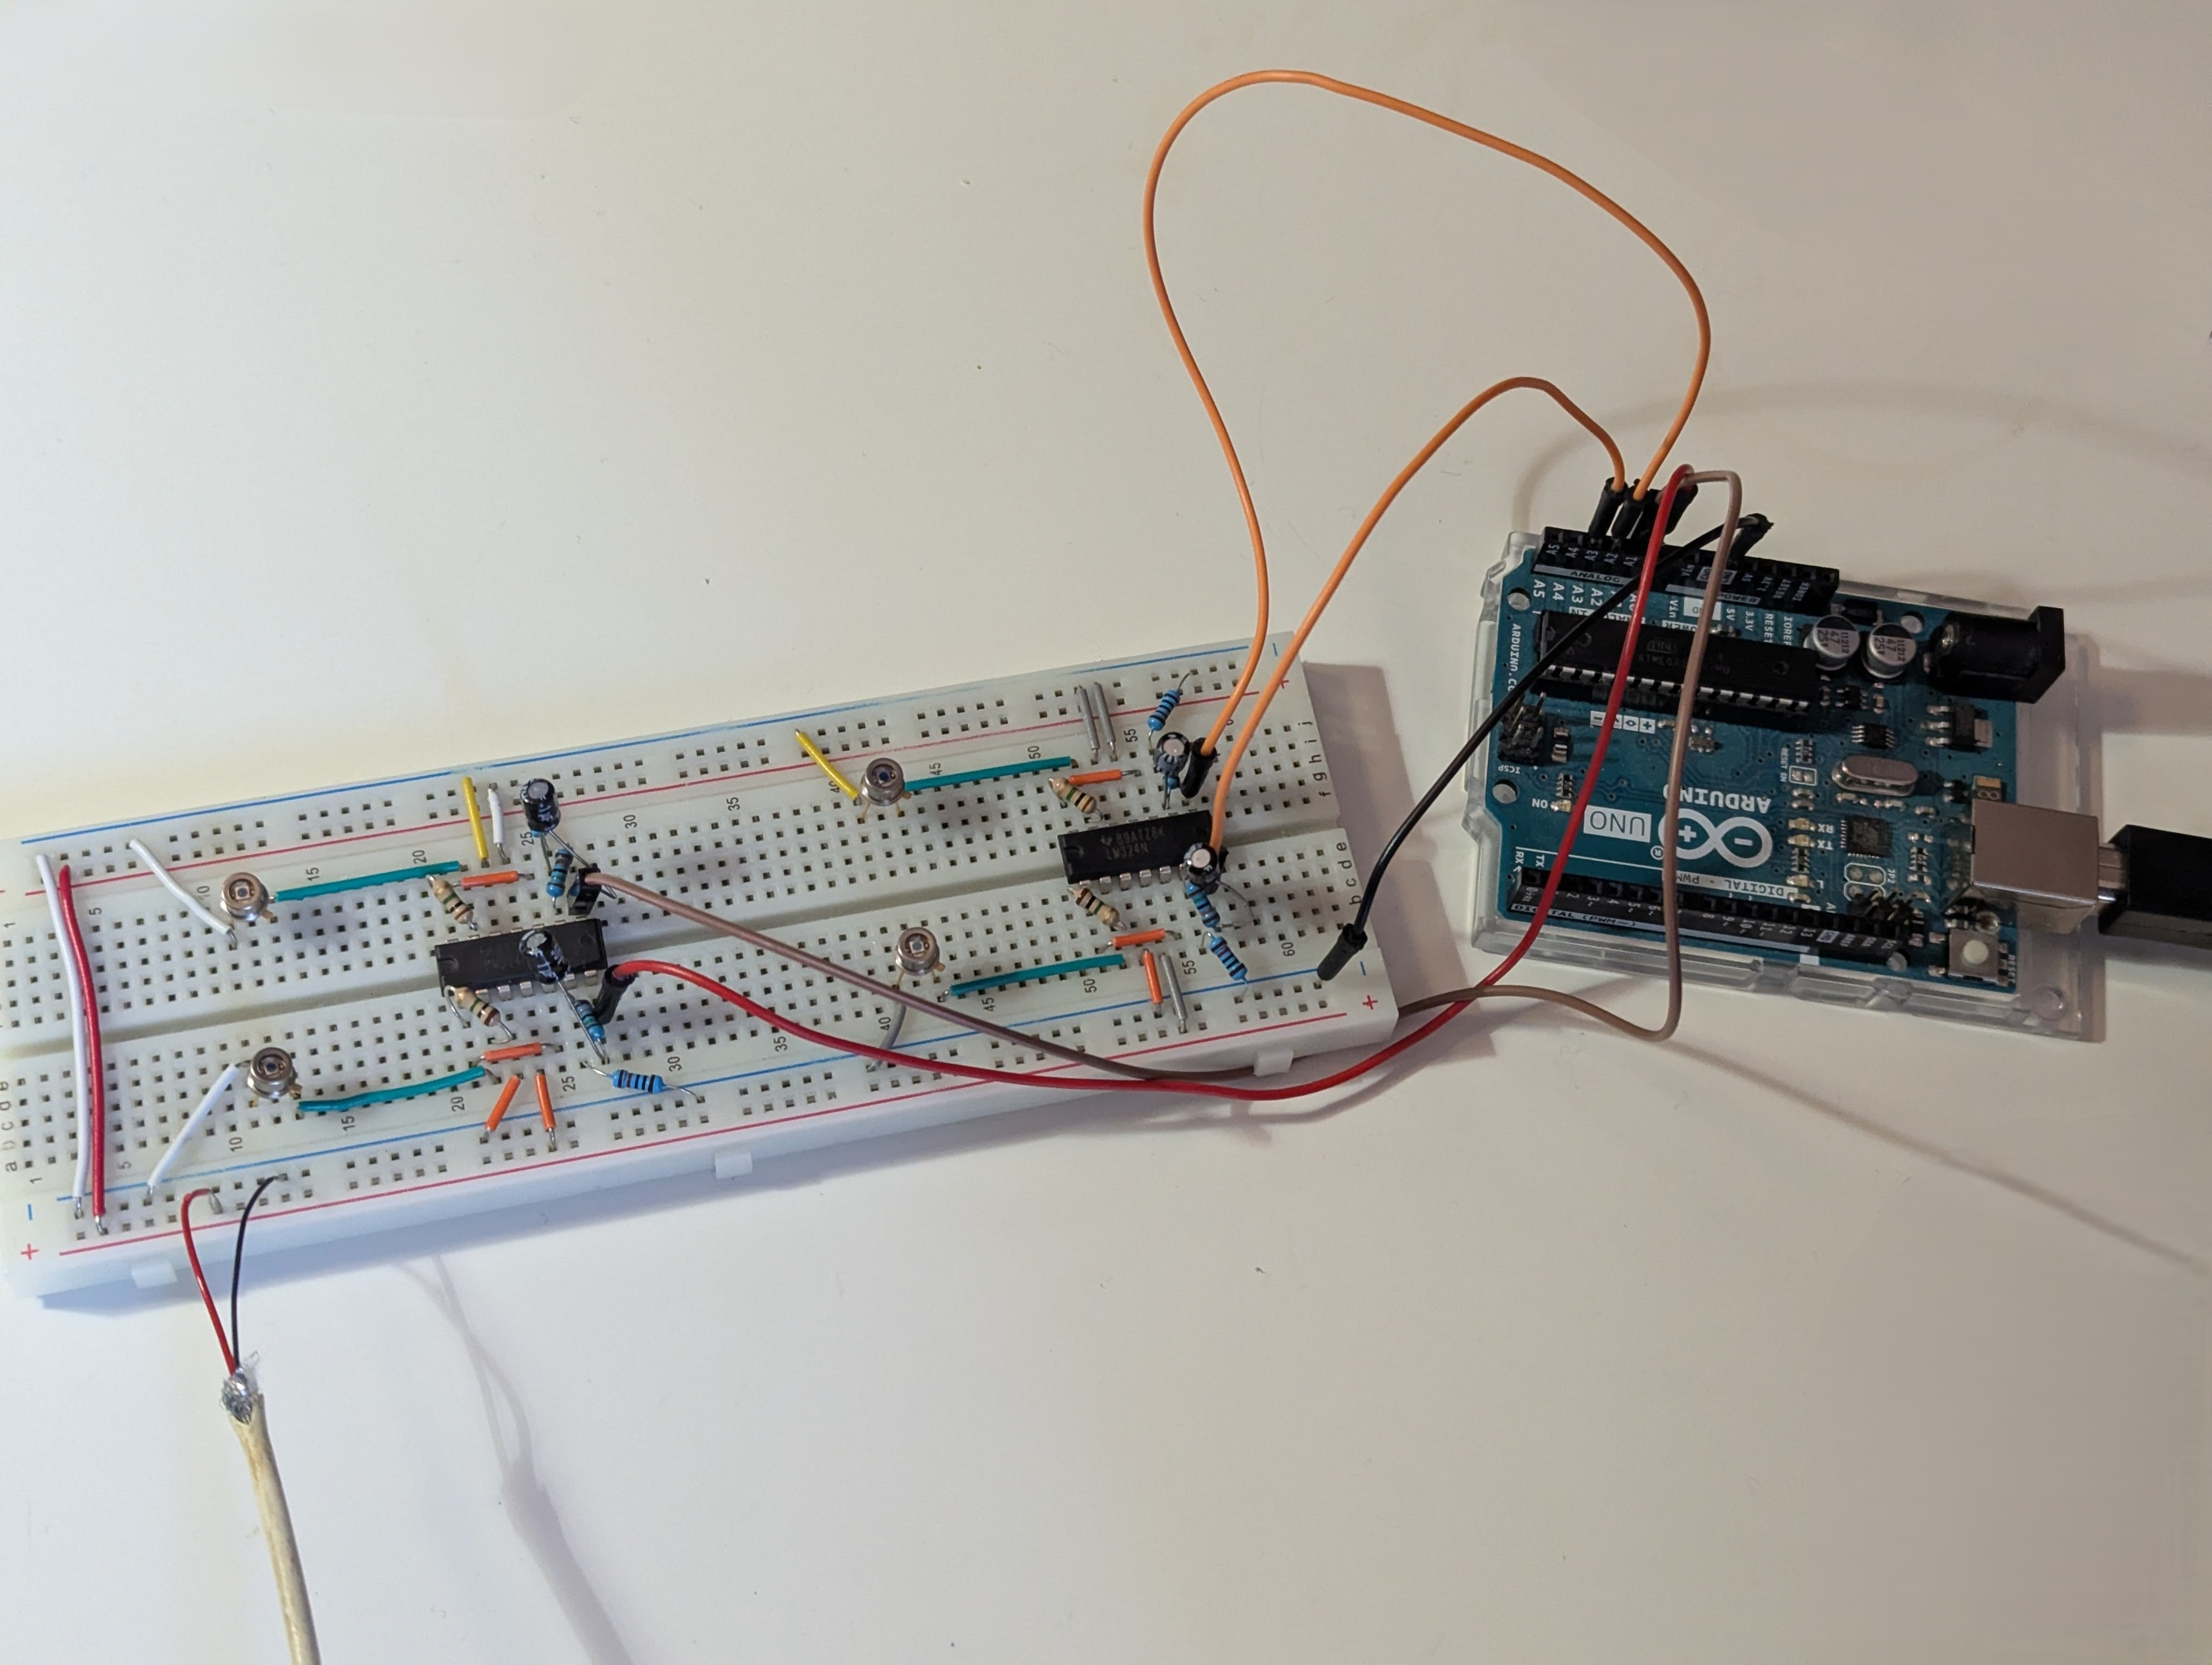
\includegraphics[width=0.8\textwidth]{chapters/methodology/prototype/BreadBoardPhoto.jpg}
  \caption{Photo Of BreadBoard Prototype}
  \label{fig:BreadBoardPhoto}
\end{figure}



\subsubsection*{Design Refinement}
\label{explainPostAmp}
\paragraph{Secondary Amplification} was added to the circuit which was a major redesign for signal conditioning. This allows reading of the analog signal with the Arduino \ac{ADC},at the full range of 0V to 5V, as the Arduino \ac{ADC} is 10 bit. This gives a resolution of  $2^{10}=1024$ steps, otherwise the readings would be from 0 V to about 300 mV, with a much lower resolution between steps - the DAQ would be using a resolution of only the region covered between 0V and 0.3V, ie. $1024/16=64$ steps. Details regarding this can be found in Section \ref{secondAmp}.
\paragraph{The Photodiodes} were first placed in a square pattern around the circuit,which helped BreadBoard prototyping but would have also simplified the Stripboard design. However, it was quickly determined that the photodides must be as close to eachother as possible, due to the light in the \ac{RED} being closer to a "single point" spreading out, as opposed to the light coming from the sun, which is assumed to be parallel. This meant that soldering the photodides to the stripboard was not an option, due to the small distance between the photodiodes and the relatively large strips on the Verooboard stripboard. The decision was therefore made to move the photodiodes to their own 3D printed enclosure, which went through it's own redisign as described under Section  



%%%%%%%%%%%%rewritten up to here ^&&&&&&&&&&&&&&&&& move this line lower when done

\begin{itemize}
  \item Optimize photodiode configuration
  \item Update signal processing algorithms
  \item Refine PCB layout
  \item Improve firmware algorithms
\end{itemize}

\subsubsection*{Stripboard Prototype Development}
%Put picture of stripboard and maybe of any measurement if available
\begin{itemize}
  \item Implementing design improvements was easy on a BreadBoard
  \item Fabricate improved aperture
  \item Enhance housing design
\end{itemize}


\subsubsection*{BreadBoard Testing}
% Stripboard photo
%
\begin{figure}[htbp] %h-ere t-op b-ottom p-page (separte) -good to allow all htbp to give the compiler more options
  \centering
  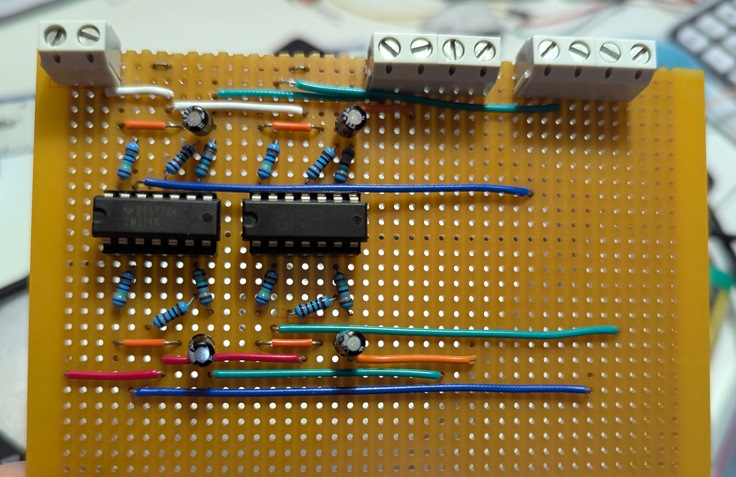
\includegraphics[width=0.7\textwidth]{chapters/methodology/prototype/StripboardPhoto.jpg}
  \caption{Photo Of Stripboard Prototype}
  \label{fig:StripboardPhoto}
\end{figure}

\subsubsection*{Comprehensive Testing}
\begin{itemize}
  \item Laboratory performance testing (angular accuracy, resolution)
  \item Improve Aperture
  \item Interface compatibility testing
\end{itemize}

\subsubsection*{Validation and Calibration}
\begin{itemize}
  \item Calibration procedure: match readings to simulation
  \item Create calibration fixtures
  \item Validate sensor performance against requirements
\end{itemize}






